\documentclass[letterpaper]{article}

% Invoke with
% pdflatex -jobname hw3-solutions "\def\showkey{}\documentclass[letterpaper]{article}

% Invoke with
% pdflatex -jobname hw3-solutions "\def\showkey{}\documentclass[letterpaper]{article}

% Invoke with
% pdflatex -jobname hw3-solutions "\def\showkey{}\documentclass[letterpaper]{article}

% Invoke with
% pdflatex -jobname hw3-solutions "\def\showkey{}\input{hw3.tex }"
% for solutions

\newif\ifkey

% \def\showkey{}

\ifdefined\showkey
  \keytrue
\else
  \keyfalse
\fi

\usepackage{hyperref}
\usepackage{tikz}
\usetikzlibrary{calc}
\usetikzlibrary{shapes}

\usepackage{fourier}
\usepackage[T1]{fontenc}
\usepackage[scaled=0.88]{luximono}
\usepackage{listings}
\lstset{language=C,
  basicstyle={\ttfamily},
}

\usepackage[top=10mm,left=11mm,right=11mm,bottom=15mm]{geometry}

% Make ``.'' a mathrel symbol: improves spacing in lambda expressions
\mathcode`\.="313A

\frenchspacing

\setlength{\pdfpageheight}{\paperheight}
\setlength{\pdfpagewidth}{\paperwidth}

\newcommand{\field}[2][]{
  \begin{tabular}{@{}c@{}}
    \fbox{\TextField[borderwidth=0,charsize=12pt,multiline=true,name={#2},#1]{}}
  \end{tabular}
  }

\title{COMS W4115 Programming Languages and Translators \\
Homework Assignment 3 \ifkey Solutions \fi}
\author{
Prof. Stephen A. Edwards \quad\quad Due Tuesday, December 4th, 2018 at 11:59 PM
}
\date{}

\pagestyle{empty}
\begin{document}
\maketitle

\ifkey\else Submit this assignment online via Courseworks as a PDF
file.  Fill in or annotate this PDF or print it out, write on it, and
scan it.  Please keep your answers in the boxes.

Do this assignment alone.  You may consult the instructor and the TAs,
but not other students.
\fi

\begin{Form}

  \medskip
  
  Name: \field[height=2pc,width=30pc,multiline=false]{name}
  Uni: \field[height=2pc,width=5pc,multiline=false,maxlen=8]{uni}

\begin{enumerate}

\item (20 pts.) For the following C array on a processor with the
  usual alignment rules,

\begin{lstlisting}
int a[2][3];
\end{lstlisting}

\begin{enumerate}
\item Show the order in which its elements are arranged in memory.

  \field[height=4pc,width=40pc]{1a}

  \ifkey
{ \raggedright
  a[0][0] \quad a[0][1] \quad a[0][2] \quad
  a[1][0] \quad a[1][1] \quad a[1][2]
  \par}

C uses row-major order: A 2D array is an array of rows.
\fi

\item Write an expression for the byte address of \verb|a[i][j]| in
  terms of $a$ (the address of the start of the array), $i$, and $j$.

    \field[height=2pc,width=40pc]{1b}

\ifkey
$a + 4(3i + j)$
\fi

\item Verify parts a) and b) by writing a small C program that
  \textbf{tests your hypothesis}.  Examine the assembly language
  output with the C compiler's \verb|-S| flag (e.g.,
  \verb|gcc -O -S array.c|).  Such a program should be simple and
  contain and access such an array, but not be so simple that the
  compiler optimizes most of it away.  On the next page,
  \textbf{include in an annotated assembly listing} that explains how
  it verifies your hypothesis.  Make sure the assembly listing is no
  more than about~40 lines, either by simplifying your program or
  trimming the output.

  C program:
  
  \field[height=16pc,width=40pc]{1c}

  \newpage

  Assembly listing:

  \field[height=9in,width=40pc]{1casm}

\ifkey
\begin{lstlisting}
int a[2][3]; /* Globals not optimized */
int i, j;    /* Make names readable */

int access() {
  return a[i][j];
}
\end{lstlisting}

\begin{verbatim}
$ gcc -O -S hw3-1.c
\end{verbatim}

\begin{verbatim}
access:
  movslq j(%rip), %rdx        ! j in %rdx
  movslq i(%rip), %rax        ! i in %rax 
  leaq   (%rax,%rax,2), %rax  ! i + 2i = 3i
  addq   %rdx, %rax           ! 3i + j
  movl   a(,%rax,4), %eax     ! a + 4(3i + j)
  ret



        .file   "hw3-1.c"
        .text
        .globl  access
        .type   access, @function
access:
.LFB0:
        .cfi_startproc
        movslq  j(%rip), %rax
        movslq  i(%rip), %rdx
        leaq    (%rdx,%rdx,2), %rdx
        addq    %rdx, %rax
        movl    a(,%rax,4), %eax
        ret
        .cfi_endproc
.LFE0:
        .size   access, .-access
        .comm   j,4,4
        .comm   i,4,4
        .comm   a,24,16
        .ident  "GCC: (Ubuntu 5.4.0-6ubuntu1~16.04.10) 5.4.0 20160609"
        .section        .note.GNU-stack,"",@progbits

\end{verbatim}
\fi

\end{enumerate}

\newpage

\item (20 pts.) For a 32-bit little-endian processor with the usual alignment
  rules, show the \textbf{memory layout} and \textbf{size in bytes} of
  the following three C variables.

  \begin{minipage}{0.3\textwidth}
\begin{lstlisting}
union {
  struct {
    char  a;  /* 8-bit */
    int   b;  /* 32-bit */
    short c;   /* 16-bit */
  } s;
  struct {
    int d;   /* 32-bit */
    short e; /* 16-bit */
  } t;
} u1;
\end{lstlisting}
  \end{minipage}%
  \begin{minipage}{0.6\textwidth}
    Layout: \field[height=6pc,width=20pc]{2a}

    \medskip
    
    Size in bytes: \field[height=2pc,width=4pc,multiline=false,maxlen=4]{2a1}
    
  \end{minipage}

  \vspace{1pc}


\ifkey%
\begin{minipage}{0.3\columnwidth}
12 bytes:

\begin{verbatim}
...a
bbbb
..cc
\end{verbatim}

or

\begin{verbatim}
dddd
..ee
\end{verbatim}
\end{minipage}
\fi

% (8 bytes)

  \begin{minipage}{0.3\textwidth}
\begin{lstlisting}
struct {
  char a;
  int b;
  short c;
  short d;
} s1;
\end{lstlisting}
  \end{minipage}%
  \begin{minipage}{0.6\textwidth}
    Layout: \field[height=6pc,width=20pc]{2b}

    \medskip
    
    Size in bytes: \field[height=2pc,width=4pc,multiline=false,maxlen=4]{2b1}
    
  \end{minipage}

\ifkey
12 bytes: \quad \begin{minipage}{0.6in}
\begin{verbatim}
...a
bbbb
ddcc
\end{verbatim}
\end{minipage}
\fi

\vspace{1pc}

\begin{minipage}{0.3\textwidth}
\begin{lstlisting}
struct {
  short a;
  char b;
  short c;
  char d;
  short e;
} s2;
\end{lstlisting}
  \end{minipage}%
  \begin{minipage}{0.6\textwidth}
    Layout: \field[height=6pc,width=20pc]{2c}

    \medskip
    
    Size in bytes: \field[height=2pc,width=4pc,multiline=false,maxlen=4]{2c1}
    
  \end{minipage}

\ifkey
10 bytes:
 \quad \begin{minipage}{0.6in}
\begin{verbatim}
.baa
.dcc
  ee
\end{verbatim}
 \end{minipage}
\fi

\item (20 pts.) Draw the layout of the stack just before \emph{bar} is called in
  \emph{foo}.  Indicate storage for function arguments, local
  variables, return addresses, and stored frame pointers.  Indicate
  where the stack and frame pointers point.

\begin{minipage}{0.5\columnwidth}
\begin{lstlisting}
void bar(int x, int y, int z);
  
void foo(int a, int b) {
  int d, e;
  bar(2, 5, 7);
}
\end{lstlisting}
\end{minipage}%
\begin{minipage}{0.5\columnwidth}
  \field[height=20pc,width=10pc]{3}
  \ifkey
\begin{tabular}{|c|l}
\\
\cline{1-1}
c \\
b \\
a \\
\cline{1-1}
ret. addr. & $\leftarrow$ fp \\
old fp \\
regs. \\
d \\
e \\
7 (z) \\
5 (y) \\
2 (x) \\
\cline{1-1}
\multicolumn{1}{c}{} & $\leftarrow$ sp \\
\end{tabular}
\fi
\end{minipage}


\newpage

\item (20 pts.)  \textbf{Draw the layouts} of s1 and s2 and the
  virtual tables for the Ellipse and Square classes.

  \begin{minipage}{0.4\textwidth}
\begin{lstlisting}[language=Java]
public class Shape {
   double x, y;
   public double area() { ... }
}

class Ellipse extends Shape {
   private double height, width;
   public double area() { ... }
}

class Square extends Shape {
   private double width;
   public double area() { ... }
}

public class Main {
  public static void main() {
    Shape s1 = new Square(10, 3, 14);
    Shape s2 = new Ellipse(3, 8, 2, 6);
    System.out.println( s1.area() );
  }
}
\end{lstlisting}
  \end{minipage}%
  \begin{minipage}{0.2\textwidth}
    Square Virtual Table:
    
    \field[height=8pc,width=8pc]{4a1}

    \vspace{2pc}
    
    s1 object:
    
    \field[height=8pc,width=8pc]{4a2}
  \end{minipage}
  \begin{minipage}{0.2\textwidth}
    Ellipse Virtual Table:
    
    \field[height=8pc,width=8pc]{4a3}

    \vspace{2pc}
    
    s2 object:
    
    \field[height=8pc,width=8pc]{4a4}
  \end{minipage}

\ifkey

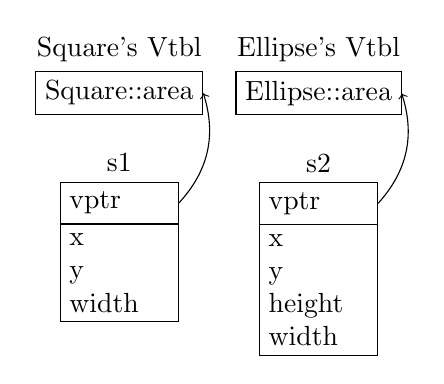
\begin{tikzpicture}[%
  object/.style={rectangle split,
                 fill=white,
                 draw
  }
]
\node [object, rectangle] (Avtbl) {
   Square::area
   };
\node [above] at (Avtbl.north) {Square's Vtbl};

\node [object, anchor=north, rectangle] (Bvtbl)
   at ($(Avtbl.north) + (right:6pc)$) {
   Ellipse::area
   };
\node [above] at (Bvtbl.north) {Ellipse's Vtbl};

\node [object, rectangle split parts=2, anchor=north,text width=3pc] (s1)
   at ($(Avtbl.south) + (down:2pc)$) { vptr \\
    \nodepart{second} x \\
 y \\
 width
};
\node [above] at (s1.north) {s1};
\draw [->] (s1.text east) to [bend right] (Avtbl.east);

\node [object, rectangle split parts=2, anchor=north,text width=3pc] (s2)
   at ($(Bvtbl.south) + (down:2pc)$) { vptr
    \nodepart{second} x \\
 y \\
 height \\
 width
    };
\node [above] at (s2.north) {s2};
\draw [->] (s2.text east) to [bend right] (Bvtbl.east);


   
\end{tikzpicture}

When \emph{area} is called, the runtime follows the object's virtual
table pointer (first field in the object) and jumps to the first
function pointer in the list (``area'').

\fi

\vspace{5pc}

\item (20 pts.)  For the program below written in a C-like language
  with nested function definitions,

  \begin{minipage}{0.4\textwidth}
\begin{lstlisting}
void main() {
  int x = 5;
  
  void bar() {
    x = x + 2;
  }
  
  void foo() {
    int x = 8;
    bar();
    printf("%d\n", x);
  }
  
  foo(); /* Body of main() */
}
\end{lstlisting}
  \end{minipage}%
  \begin{minipage}{0.6\textwidth}
    What would it print if the language used \textbf{static scoping}?   
    \field[height=3pc,width=3pc,multiline=false]{5a}

    \vspace{2pc}

    What would it print if the language used \textbf{dynamic scoping}?    
    \field[height=3pc,width=3pc,multiline=false]{5b}
  \end{minipage}

\ifkey
Static scoping: 8 \quad \emph{bar} doesn't change local \emph{x}\\
Dynamic scoping: 10 \quad \emph{bar} changes 8 into 10 \\
\fi

\end{enumerate}

\end{Form}

\end{document}

% Local Variables:
% compile-command: "make hw3.pdf"
% End:
"
% for solutions

\newif\ifkey

% \def\showkey{}

\ifdefined\showkey
  \keytrue
\else
  \keyfalse
\fi

\usepackage{hyperref}
\usepackage{tikz}
\usetikzlibrary{calc}
\usetikzlibrary{shapes}

\usepackage{fourier}
\usepackage[T1]{fontenc}
\usepackage[scaled=0.88]{luximono}
\usepackage{listings}
\lstset{language=C,
  basicstyle={\ttfamily},
}

\usepackage[top=10mm,left=11mm,right=11mm,bottom=15mm]{geometry}

% Make ``.'' a mathrel symbol: improves spacing in lambda expressions
\mathcode`\.="313A

\frenchspacing

\setlength{\pdfpageheight}{\paperheight}
\setlength{\pdfpagewidth}{\paperwidth}

\newcommand{\field}[2][]{
  \begin{tabular}{@{}c@{}}
    \fbox{\TextField[borderwidth=0,charsize=12pt,multiline=true,name={#2},#1]{}}
  \end{tabular}
  }

\title{COMS W4115 Programming Languages and Translators \\
Homework Assignment 3 \ifkey Solutions \fi}
\author{
Prof. Stephen A. Edwards \quad\quad Due Tuesday, December 4th, 2018 at 11:59 PM
}
\date{}

\pagestyle{empty}
\begin{document}
\maketitle

\ifkey\else Submit this assignment online via Courseworks as a PDF
file.  Fill in or annotate this PDF or print it out, write on it, and
scan it.  Please keep your answers in the boxes.

Do this assignment alone.  You may consult the instructor and the TAs,
but not other students.
\fi

\begin{Form}

  \medskip
  
  Name: \field[height=2pc,width=30pc,multiline=false]{name}
  Uni: \field[height=2pc,width=5pc,multiline=false,maxlen=8]{uni}

\begin{enumerate}

\item (20 pts.) For the following C array on a processor with the
  usual alignment rules,

\begin{lstlisting}
int a[2][3];
\end{lstlisting}

\begin{enumerate}
\item Show the order in which its elements are arranged in memory.

  \field[height=4pc,width=40pc]{1a}

  \ifkey
{ \raggedright
  a[0][0] \quad a[0][1] \quad a[0][2] \quad
  a[1][0] \quad a[1][1] \quad a[1][2]
  \par}

C uses row-major order: A 2D array is an array of rows.
\fi

\item Write an expression for the byte address of \verb|a[i][j]| in
  terms of $a$ (the address of the start of the array), $i$, and $j$.

    \field[height=2pc,width=40pc]{1b}

\ifkey
$a + 4(3i + j)$
\fi

\item Verify parts a) and b) by writing a small C program that
  \textbf{tests your hypothesis}.  Examine the assembly language
  output with the C compiler's \verb|-S| flag (e.g.,
  \verb|gcc -O -S array.c|).  Such a program should be simple and
  contain and access such an array, but not be so simple that the
  compiler optimizes most of it away.  On the next page,
  \textbf{include in an annotated assembly listing} that explains how
  it verifies your hypothesis.  Make sure the assembly listing is no
  more than about~40 lines, either by simplifying your program or
  trimming the output.

  C program:
  
  \field[height=16pc,width=40pc]{1c}

  \newpage

  Assembly listing:

  \field[height=9in,width=40pc]{1casm}

\ifkey
\begin{lstlisting}
int a[2][3]; /* Globals not optimized */
int i, j;    /* Make names readable */

int access() {
  return a[i][j];
}
\end{lstlisting}

\begin{verbatim}
$ gcc -O -S hw3-1.c
\end{verbatim}

\begin{verbatim}
access:
  movslq j(%rip), %rdx        ! j in %rdx
  movslq i(%rip), %rax        ! i in %rax 
  leaq   (%rax,%rax,2), %rax  ! i + 2i = 3i
  addq   %rdx, %rax           ! 3i + j
  movl   a(,%rax,4), %eax     ! a + 4(3i + j)
  ret



        .file   "hw3-1.c"
        .text
        .globl  access
        .type   access, @function
access:
.LFB0:
        .cfi_startproc
        movslq  j(%rip), %rax
        movslq  i(%rip), %rdx
        leaq    (%rdx,%rdx,2), %rdx
        addq    %rdx, %rax
        movl    a(,%rax,4), %eax
        ret
        .cfi_endproc
.LFE0:
        .size   access, .-access
        .comm   j,4,4
        .comm   i,4,4
        .comm   a,24,16
        .ident  "GCC: (Ubuntu 5.4.0-6ubuntu1~16.04.10) 5.4.0 20160609"
        .section        .note.GNU-stack,"",@progbits

\end{verbatim}
\fi

\end{enumerate}

\newpage

\item (20 pts.) For a 32-bit little-endian processor with the usual alignment
  rules, show the \textbf{memory layout} and \textbf{size in bytes} of
  the following three C variables.

  \begin{minipage}{0.3\textwidth}
\begin{lstlisting}
union {
  struct {
    char  a;  /* 8-bit */
    int   b;  /* 32-bit */
    short c;   /* 16-bit */
  } s;
  struct {
    int d;   /* 32-bit */
    short e; /* 16-bit */
  } t;
} u1;
\end{lstlisting}
  \end{minipage}%
  \begin{minipage}{0.6\textwidth}
    Layout: \field[height=6pc,width=20pc]{2a}

    \medskip
    
    Size in bytes: \field[height=2pc,width=4pc,multiline=false,maxlen=4]{2a1}
    
  \end{minipage}

  \vspace{1pc}


\ifkey%
\begin{minipage}{0.3\columnwidth}
12 bytes:

\begin{verbatim}
...a
bbbb
..cc
\end{verbatim}

or

\begin{verbatim}
dddd
..ee
\end{verbatim}
\end{minipage}
\fi

% (8 bytes)

  \begin{minipage}{0.3\textwidth}
\begin{lstlisting}
struct {
  char a;
  int b;
  short c;
  short d;
} s1;
\end{lstlisting}
  \end{minipage}%
  \begin{minipage}{0.6\textwidth}
    Layout: \field[height=6pc,width=20pc]{2b}

    \medskip
    
    Size in bytes: \field[height=2pc,width=4pc,multiline=false,maxlen=4]{2b1}
    
  \end{minipage}

\ifkey
12 bytes: \quad \begin{minipage}{0.6in}
\begin{verbatim}
...a
bbbb
ddcc
\end{verbatim}
\end{minipage}
\fi

\vspace{1pc}

\begin{minipage}{0.3\textwidth}
\begin{lstlisting}
struct {
  short a;
  char b;
  short c;
  char d;
  short e;
} s2;
\end{lstlisting}
  \end{minipage}%
  \begin{minipage}{0.6\textwidth}
    Layout: \field[height=6pc,width=20pc]{2c}

    \medskip
    
    Size in bytes: \field[height=2pc,width=4pc,multiline=false,maxlen=4]{2c1}
    
  \end{minipage}

\ifkey
10 bytes:
 \quad \begin{minipage}{0.6in}
\begin{verbatim}
.baa
.dcc
  ee
\end{verbatim}
 \end{minipage}
\fi

\item (20 pts.) Draw the layout of the stack just before \emph{bar} is called in
  \emph{foo}.  Indicate storage for function arguments, local
  variables, return addresses, and stored frame pointers.  Indicate
  where the stack and frame pointers point.

\begin{minipage}{0.5\columnwidth}
\begin{lstlisting}
void bar(int x, int y, int z);
  
void foo(int a, int b) {
  int d, e;
  bar(2, 5, 7);
}
\end{lstlisting}
\end{minipage}%
\begin{minipage}{0.5\columnwidth}
  \field[height=20pc,width=10pc]{3}
  \ifkey
\begin{tabular}{|c|l}
\\
\cline{1-1}
c \\
b \\
a \\
\cline{1-1}
ret. addr. & $\leftarrow$ fp \\
old fp \\
regs. \\
d \\
e \\
7 (z) \\
5 (y) \\
2 (x) \\
\cline{1-1}
\multicolumn{1}{c}{} & $\leftarrow$ sp \\
\end{tabular}
\fi
\end{minipage}


\newpage

\item (20 pts.)  \textbf{Draw the layouts} of s1 and s2 and the
  virtual tables for the Ellipse and Square classes.

  \begin{minipage}{0.4\textwidth}
\begin{lstlisting}[language=Java]
public class Shape {
   double x, y;
   public double area() { ... }
}

class Ellipse extends Shape {
   private double height, width;
   public double area() { ... }
}

class Square extends Shape {
   private double width;
   public double area() { ... }
}

public class Main {
  public static void main() {
    Shape s1 = new Square(10, 3, 14);
    Shape s2 = new Ellipse(3, 8, 2, 6);
    System.out.println( s1.area() );
  }
}
\end{lstlisting}
  \end{minipage}%
  \begin{minipage}{0.2\textwidth}
    Square Virtual Table:
    
    \field[height=8pc,width=8pc]{4a1}

    \vspace{2pc}
    
    s1 object:
    
    \field[height=8pc,width=8pc]{4a2}
  \end{minipage}
  \begin{minipage}{0.2\textwidth}
    Ellipse Virtual Table:
    
    \field[height=8pc,width=8pc]{4a3}

    \vspace{2pc}
    
    s2 object:
    
    \field[height=8pc,width=8pc]{4a4}
  \end{minipage}

\ifkey

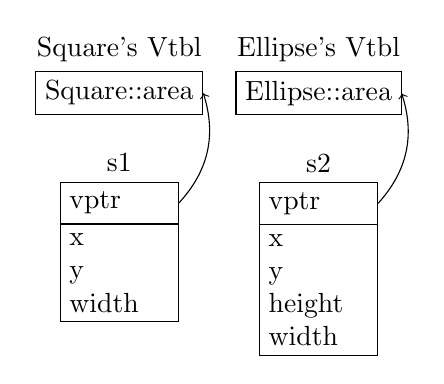
\begin{tikzpicture}[%
  object/.style={rectangle split,
                 fill=white,
                 draw
  }
]
\node [object, rectangle] (Avtbl) {
   Square::area
   };
\node [above] at (Avtbl.north) {Square's Vtbl};

\node [object, anchor=north, rectangle] (Bvtbl)
   at ($(Avtbl.north) + (right:6pc)$) {
   Ellipse::area
   };
\node [above] at (Bvtbl.north) {Ellipse's Vtbl};

\node [object, rectangle split parts=2, anchor=north,text width=3pc] (s1)
   at ($(Avtbl.south) + (down:2pc)$) { vptr \\
    \nodepart{second} x \\
 y \\
 width
};
\node [above] at (s1.north) {s1};
\draw [->] (s1.text east) to [bend right] (Avtbl.east);

\node [object, rectangle split parts=2, anchor=north,text width=3pc] (s2)
   at ($(Bvtbl.south) + (down:2pc)$) { vptr
    \nodepart{second} x \\
 y \\
 height \\
 width
    };
\node [above] at (s2.north) {s2};
\draw [->] (s2.text east) to [bend right] (Bvtbl.east);


   
\end{tikzpicture}

When \emph{area} is called, the runtime follows the object's virtual
table pointer (first field in the object) and jumps to the first
function pointer in the list (``area'').

\fi

\vspace{5pc}

\item (20 pts.)  For the program below written in a C-like language
  with nested function definitions,

  \begin{minipage}{0.4\textwidth}
\begin{lstlisting}
void main() {
  int x = 5;
  
  void bar() {
    x = x + 2;
  }
  
  void foo() {
    int x = 8;
    bar();
    printf("%d\n", x);
  }
  
  foo(); /* Body of main() */
}
\end{lstlisting}
  \end{minipage}%
  \begin{minipage}{0.6\textwidth}
    What would it print if the language used \textbf{static scoping}?   
    \field[height=3pc,width=3pc,multiline=false]{5a}

    \vspace{2pc}

    What would it print if the language used \textbf{dynamic scoping}?    
    \field[height=3pc,width=3pc,multiline=false]{5b}
  \end{minipage}

\ifkey
Static scoping: 8 \quad \emph{bar} doesn't change local \emph{x}\\
Dynamic scoping: 10 \quad \emph{bar} changes 8 into 10 \\
\fi

\end{enumerate}

\end{Form}

\end{document}

% Local Variables:
% compile-command: "make hw3.pdf"
% End:
"
% for solutions

\newif\ifkey

% \def\showkey{}

\ifdefined\showkey
  \keytrue
\else
  \keyfalse
\fi

\usepackage{hyperref}
\usepackage{tikz}
\usetikzlibrary{calc}
\usetikzlibrary{shapes}

\usepackage{fourier}
\usepackage[T1]{fontenc}
\usepackage[scaled=0.88]{luximono}
\usepackage{listings}
\lstset{language=C,
  basicstyle={\ttfamily},
}

\usepackage[top=10mm,left=11mm,right=11mm,bottom=15mm]{geometry}

% Make ``.'' a mathrel symbol: improves spacing in lambda expressions
\mathcode`\.="313A

\frenchspacing

\setlength{\pdfpageheight}{\paperheight}
\setlength{\pdfpagewidth}{\paperwidth}

\newcommand{\field}[2][]{
  \begin{tabular}{@{}c@{}}
    \fbox{\TextField[borderwidth=0,charsize=12pt,multiline=true,name={#2},#1]{}}
  \end{tabular}
  }

\title{COMS W4115 Programming Languages and Translators \\
Homework Assignment 3 \ifkey Solutions \fi}
\author{
Prof. Stephen A. Edwards \quad\quad Due Tuesday, December 4th, 2018 at 11:59 PM
}
\date{}

\pagestyle{empty}
\begin{document}
\maketitle

\ifkey\else Submit this assignment online via Courseworks as a PDF
file.  Fill in or annotate this PDF or print it out, write on it, and
scan it.  Please keep your answers in the boxes.

Do this assignment alone.  You may consult the instructor and the TAs,
but not other students.
\fi

\begin{Form}

  \medskip
  
  Name: \field[height=2pc,width=30pc,multiline=false]{name}
  Uni: \field[height=2pc,width=5pc,multiline=false,maxlen=8]{uni}

\begin{enumerate}

\item (20 pts.) For the following C array on a processor with the
  usual alignment rules,

\begin{lstlisting}
int a[2][3];
\end{lstlisting}

\begin{enumerate}
\item Show the order in which its elements are arranged in memory.

  \field[height=4pc,width=40pc]{1a}

  \ifkey
{ \raggedright
  a[0][0] \quad a[0][1] \quad a[0][2] \quad
  a[1][0] \quad a[1][1] \quad a[1][2]
  \par}

C uses row-major order: A 2D array is an array of rows.
\fi

\item Write an expression for the byte address of \verb|a[i][j]| in
  terms of $a$ (the address of the start of the array), $i$, and $j$.

    \field[height=2pc,width=40pc]{1b}

\ifkey
$a + 4(3i + j)$
\fi

\item Verify parts a) and b) by writing a small C program that
  \textbf{tests your hypothesis}.  Examine the assembly language
  output with the C compiler's \verb|-S| flag (e.g.,
  \verb|gcc -O -S array.c|).  Such a program should be simple and
  contain and access such an array, but not be so simple that the
  compiler optimizes most of it away.  On the next page,
  \textbf{include in an annotated assembly listing} that explains how
  it verifies your hypothesis.  Make sure the assembly listing is no
  more than about~40 lines, either by simplifying your program or
  trimming the output.

  C program:
  
  \field[height=16pc,width=40pc]{1c}

  \newpage

  Assembly listing:

  \field[height=9in,width=40pc]{1casm}

\ifkey
\begin{lstlisting}
int a[2][3]; /* Globals not optimized */
int i, j;    /* Make names readable */

int access() {
  return a[i][j];
}
\end{lstlisting}

\begin{verbatim}
$ gcc -O -S hw3-1.c
\end{verbatim}

\begin{verbatim}
access:
  movslq j(%rip), %rdx        ! j in %rdx
  movslq i(%rip), %rax        ! i in %rax 
  leaq   (%rax,%rax,2), %rax  ! i + 2i = 3i
  addq   %rdx, %rax           ! 3i + j
  movl   a(,%rax,4), %eax     ! a + 4(3i + j)
  ret



        .file   "hw3-1.c"
        .text
        .globl  access
        .type   access, @function
access:
.LFB0:
        .cfi_startproc
        movslq  j(%rip), %rax
        movslq  i(%rip), %rdx
        leaq    (%rdx,%rdx,2), %rdx
        addq    %rdx, %rax
        movl    a(,%rax,4), %eax
        ret
        .cfi_endproc
.LFE0:
        .size   access, .-access
        .comm   j,4,4
        .comm   i,4,4
        .comm   a,24,16
        .ident  "GCC: (Ubuntu 5.4.0-6ubuntu1~16.04.10) 5.4.0 20160609"
        .section        .note.GNU-stack,"",@progbits

\end{verbatim}
\fi

\end{enumerate}

\newpage

\item (20 pts.) For a 32-bit little-endian processor with the usual alignment
  rules, show the \textbf{memory layout} and \textbf{size in bytes} of
  the following three C variables.

  \begin{minipage}{0.3\textwidth}
\begin{lstlisting}
union {
  struct {
    char  a;  /* 8-bit */
    int   b;  /* 32-bit */
    short c;   /* 16-bit */
  } s;
  struct {
    int d;   /* 32-bit */
    short e; /* 16-bit */
  } t;
} u1;
\end{lstlisting}
  \end{minipage}%
  \begin{minipage}{0.6\textwidth}
    Layout: \field[height=6pc,width=20pc]{2a}

    \medskip
    
    Size in bytes: \field[height=2pc,width=4pc,multiline=false,maxlen=4]{2a1}
    
  \end{minipage}

  \vspace{1pc}


\ifkey%
\begin{minipage}{0.3\columnwidth}
12 bytes:

\begin{verbatim}
...a
bbbb
..cc
\end{verbatim}

or

\begin{verbatim}
dddd
..ee
\end{verbatim}
\end{minipage}
\fi

% (8 bytes)

  \begin{minipage}{0.3\textwidth}
\begin{lstlisting}
struct {
  char a;
  int b;
  short c;
  short d;
} s1;
\end{lstlisting}
  \end{minipage}%
  \begin{minipage}{0.6\textwidth}
    Layout: \field[height=6pc,width=20pc]{2b}

    \medskip
    
    Size in bytes: \field[height=2pc,width=4pc,multiline=false,maxlen=4]{2b1}
    
  \end{minipage}

\ifkey
12 bytes: \quad \begin{minipage}{0.6in}
\begin{verbatim}
...a
bbbb
ddcc
\end{verbatim}
\end{minipage}
\fi

\vspace{1pc}

\begin{minipage}{0.3\textwidth}
\begin{lstlisting}
struct {
  short a;
  char b;
  short c;
  char d;
  short e;
} s2;
\end{lstlisting}
  \end{minipage}%
  \begin{minipage}{0.6\textwidth}
    Layout: \field[height=6pc,width=20pc]{2c}

    \medskip
    
    Size in bytes: \field[height=2pc,width=4pc,multiline=false,maxlen=4]{2c1}
    
  \end{minipage}

\ifkey
10 bytes:
 \quad \begin{minipage}{0.6in}
\begin{verbatim}
.baa
.dcc
  ee
\end{verbatim}
 \end{minipage}
\fi

\item (20 pts.) Draw the layout of the stack just before \emph{bar} is called in
  \emph{foo}.  Indicate storage for function arguments, local
  variables, return addresses, and stored frame pointers.  Indicate
  where the stack and frame pointers point.

\begin{minipage}{0.5\columnwidth}
\begin{lstlisting}
void bar(int x, int y, int z);
  
void foo(int a, int b) {
  int d, e;
  bar(2, 5, 7);
}
\end{lstlisting}
\end{minipage}%
\begin{minipage}{0.5\columnwidth}
  \field[height=20pc,width=10pc]{3}
  \ifkey
\begin{tabular}{|c|l}
\\
\cline{1-1}
c \\
b \\
a \\
\cline{1-1}
ret. addr. & $\leftarrow$ fp \\
old fp \\
regs. \\
d \\
e \\
7 (z) \\
5 (y) \\
2 (x) \\
\cline{1-1}
\multicolumn{1}{c}{} & $\leftarrow$ sp \\
\end{tabular}
\fi
\end{minipage}


\newpage

\item (20 pts.)  \textbf{Draw the layouts} of s1 and s2 and the
  virtual tables for the Ellipse and Square classes.

  \begin{minipage}{0.4\textwidth}
\begin{lstlisting}[language=Java]
public class Shape {
   double x, y;
   public double area() { ... }
}

class Ellipse extends Shape {
   private double height, width;
   public double area() { ... }
}

class Square extends Shape {
   private double width;
   public double area() { ... }
}

public class Main {
  public static void main() {
    Shape s1 = new Square(10, 3, 14);
    Shape s2 = new Ellipse(3, 8, 2, 6);
    System.out.println( s1.area() );
  }
}
\end{lstlisting}
  \end{minipage}%
  \begin{minipage}{0.2\textwidth}
    Square Virtual Table:
    
    \field[height=8pc,width=8pc]{4a1}

    \vspace{2pc}
    
    s1 object:
    
    \field[height=8pc,width=8pc]{4a2}
  \end{minipage}
  \begin{minipage}{0.2\textwidth}
    Ellipse Virtual Table:
    
    \field[height=8pc,width=8pc]{4a3}

    \vspace{2pc}
    
    s2 object:
    
    \field[height=8pc,width=8pc]{4a4}
  \end{minipage}

\ifkey

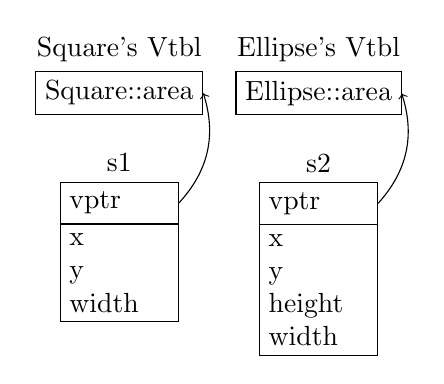
\begin{tikzpicture}[%
  object/.style={rectangle split,
                 fill=white,
                 draw
  }
]
\node [object, rectangle] (Avtbl) {
   Square::area
   };
\node [above] at (Avtbl.north) {Square's Vtbl};

\node [object, anchor=north, rectangle] (Bvtbl)
   at ($(Avtbl.north) + (right:6pc)$) {
   Ellipse::area
   };
\node [above] at (Bvtbl.north) {Ellipse's Vtbl};

\node [object, rectangle split parts=2, anchor=north,text width=3pc] (s1)
   at ($(Avtbl.south) + (down:2pc)$) { vptr \\
    \nodepart{second} x \\
 y \\
 width
};
\node [above] at (s1.north) {s1};
\draw [->] (s1.text east) to [bend right] (Avtbl.east);

\node [object, rectangle split parts=2, anchor=north,text width=3pc] (s2)
   at ($(Bvtbl.south) + (down:2pc)$) { vptr
    \nodepart{second} x \\
 y \\
 height \\
 width
    };
\node [above] at (s2.north) {s2};
\draw [->] (s2.text east) to [bend right] (Bvtbl.east);


   
\end{tikzpicture}

When \emph{area} is called, the runtime follows the object's virtual
table pointer (first field in the object) and jumps to the first
function pointer in the list (``area'').

\fi

\vspace{5pc}

\item (20 pts.)  For the program below written in a C-like language
  with nested function definitions,

  \begin{minipage}{0.4\textwidth}
\begin{lstlisting}
void main() {
  int x = 5;
  
  void bar() {
    x = x + 2;
  }
  
  void foo() {
    int x = 8;
    bar();
    printf("%d\n", x);
  }
  
  foo(); /* Body of main() */
}
\end{lstlisting}
  \end{minipage}%
  \begin{minipage}{0.6\textwidth}
    What would it print if the language used \textbf{static scoping}?   
    \field[height=3pc,width=3pc,multiline=false]{5a}

    \vspace{2pc}

    What would it print if the language used \textbf{dynamic scoping}?    
    \field[height=3pc,width=3pc,multiline=false]{5b}
  \end{minipage}

\ifkey
Static scoping: 8 \quad \emph{bar} doesn't change local \emph{x}\\
Dynamic scoping: 10 \quad \emph{bar} changes 8 into 10 \\
\fi

\end{enumerate}

\end{Form}

\end{document}

% Local Variables:
% compile-command: "make hw3.pdf"
% End:
"
% for solutions

\newif\ifkey

% \def\showkey{}

\ifdefined\showkey
  \keytrue
\else
  \keyfalse
\fi

\usepackage{hyperref}
\usepackage{tikz}
\usetikzlibrary{calc}
\usetikzlibrary{shapes}

\usepackage{fourier}
\usepackage[T1]{fontenc}
\usepackage[scaled=0.88]{luximono}
\usepackage{listings}
\lstset{language=C,
  basicstyle={\ttfamily},
}

\usepackage[top=10mm,left=11mm,right=11mm,bottom=15mm]{geometry}

% Make ``.'' a mathrel symbol: improves spacing in lambda expressions
\mathcode`\.="313A

\frenchspacing

\setlength{\pdfpageheight}{\paperheight}
\setlength{\pdfpagewidth}{\paperwidth}

\newcommand{\field}[2][]{
  \begin{tabular}{@{}c@{}}
    \fbox{\TextField[borderwidth=0,charsize=12pt,multiline=true,name={#2},#1]{}}
  \end{tabular}
  }

\title{COMS W4115 Programming Languages and Translators \\
Homework Assignment 3 \ifkey Solutions \fi}
\author{
Prof. Stephen A. Edwards \quad\quad Due Tuesday, December 4th, 2018 at 11:59 PM
}
\date{}

\pagestyle{empty}
\begin{document}
\maketitle

\ifkey\else Submit this assignment online via Courseworks as a PDF
file.  Fill in or annotate this PDF or print it out, write on it, and
scan it.  Please keep your answers in the boxes.

Do this assignment alone.  You may consult the instructor and the TAs,
but not other students.
\fi

\begin{Form}

  \medskip
  
  Name: \field[height=2pc,width=30pc,multiline=false]{name}
  Uni: \field[height=2pc,width=5pc,multiline=false,maxlen=8]{uni}

\begin{enumerate}

\item (20 pts.) For the following C array on a processor with the
  usual alignment rules,

\begin{lstlisting}
int a[2][3];
\end{lstlisting}

\begin{enumerate}
\item Show the order in which its elements are arranged in memory.

  \field[height=4pc,width=40pc]{1a}

  \ifkey
{ \raggedright
  a[0][0] \quad a[0][1] \quad a[0][2] \quad
  a[1][0] \quad a[1][1] \quad a[1][2]
  \par}

C uses row-major order: A 2D array is an array of rows.
\fi

\item Write an expression for the byte address of \verb|a[i][j]| in
  terms of $a$ (the address of the start of the array), $i$, and $j$.

    \field[height=2pc,width=40pc]{1b}

\ifkey
$a + 4(3i + j)$
\fi

\item Verify parts a) and b) by writing a small C program that
  \textbf{tests your hypothesis}.  Examine the assembly language
  output with the C compiler's \verb|-S| flag (e.g.,
  \verb|gcc -O -S array.c|).  Such a program should be simple and
  contain and access such an array, but not be so simple that the
  compiler optimizes most of it away.  On the next page,
  \textbf{include in an annotated assembly listing} that explains how
  it verifies your hypothesis.  Make sure the assembly listing is no
  more than about~40 lines, either by simplifying your program or
  trimming the output.

  C program:
  
  \field[height=16pc,width=40pc]{1c}

  \newpage

  Assembly listing:

  \field[height=9in,width=40pc]{1casm}

\ifkey
\begin{lstlisting}
int a[2][3]; /* Globals not optimized */
int i, j;    /* Make names readable */

int access() {
  return a[i][j];
}
\end{lstlisting}

\begin{verbatim}
$ gcc -O -S hw3-1.c
\end{verbatim}

\begin{verbatim}
access:
  movslq j(%rip), %rdx        ! j in %rdx
  movslq i(%rip), %rax        ! i in %rax 
  leaq   (%rax,%rax,2), %rax  ! i + 2i = 3i
  addq   %rdx, %rax           ! 3i + j
  movl   a(,%rax,4), %eax     ! a + 4(3i + j)
  ret



        .file   "hw3-1.c"
        .text
        .globl  access
        .type   access, @function
access:
.LFB0:
        .cfi_startproc
        movslq  j(%rip), %rax
        movslq  i(%rip), %rdx
        leaq    (%rdx,%rdx,2), %rdx
        addq    %rdx, %rax
        movl    a(,%rax,4), %eax
        ret
        .cfi_endproc
.LFE0:
        .size   access, .-access
        .comm   j,4,4
        .comm   i,4,4
        .comm   a,24,16
        .ident  "GCC: (Ubuntu 5.4.0-6ubuntu1~16.04.10) 5.4.0 20160609"
        .section        .note.GNU-stack,"",@progbits

\end{verbatim}
\fi

\end{enumerate}

\newpage

\item (20 pts.) For a 32-bit little-endian processor with the usual alignment
  rules, show the \textbf{memory layout} and \textbf{size in bytes} of
  the following three C variables.

  \begin{minipage}{0.3\textwidth}
\begin{lstlisting}
union {
  struct {
    char  a;  /* 8-bit */
    int   b;  /* 32-bit */
    short c;   /* 16-bit */
  } s;
  struct {
    int d;   /* 32-bit */
    short e; /* 16-bit */
  } t;
} u1;
\end{lstlisting}
  \end{minipage}%
  \begin{minipage}{0.6\textwidth}
    Layout: \field[height=6pc,width=20pc]{2a}

    \medskip
    
    Size in bytes: \field[height=2pc,width=4pc,multiline=false,maxlen=4]{2a1}
    
  \end{minipage}

  \vspace{1pc}


\ifkey%
\begin{minipage}{0.3\columnwidth}
12 bytes:

\begin{verbatim}
...a
bbbb
..cc
\end{verbatim}

or

\begin{verbatim}
dddd
..ee
\end{verbatim}
\end{minipage}
\fi

% (8 bytes)

  \begin{minipage}{0.3\textwidth}
\begin{lstlisting}
struct {
  char a;
  int b;
  short c;
  short d;
} s1;
\end{lstlisting}
  \end{minipage}%
  \begin{minipage}{0.6\textwidth}
    Layout: \field[height=6pc,width=20pc]{2b}

    \medskip
    
    Size in bytes: \field[height=2pc,width=4pc,multiline=false,maxlen=4]{2b1}
    
  \end{minipage}

\ifkey
12 bytes: \quad \begin{minipage}{0.6in}
\begin{verbatim}
...a
bbbb
ddcc
\end{verbatim}
\end{minipage}
\fi

\vspace{1pc}

\begin{minipage}{0.3\textwidth}
\begin{lstlisting}
struct {
  short a;
  char b;
  short c;
  char d;
  short e;
} s2;
\end{lstlisting}
  \end{minipage}%
  \begin{minipage}{0.6\textwidth}
    Layout: \field[height=6pc,width=20pc]{2c}

    \medskip
    
    Size in bytes: \field[height=2pc,width=4pc,multiline=false,maxlen=4]{2c1}
    
  \end{minipage}

\ifkey
10 bytes:
 \quad \begin{minipage}{0.6in}
\begin{verbatim}
.baa
.dcc
  ee
\end{verbatim}
 \end{minipage}
\fi

\item (20 pts.) Draw the layout of the stack just before \emph{bar} is called in
  \emph{foo}.  Indicate storage for function arguments, local
  variables, return addresses, and stored frame pointers.  Indicate
  where the stack and frame pointers point.

\begin{minipage}{0.5\columnwidth}
\begin{lstlisting}
void bar(int x, int y, int z);
  
void foo(int a, int b) {
  int d, e;
  bar(2, 5, 7);
}
\end{lstlisting}
\end{minipage}%
\begin{minipage}{0.5\columnwidth}
  \field[height=20pc,width=10pc]{3}
  \ifkey
\begin{tabular}{|c|l}
\\
\cline{1-1}
c \\
b \\
a \\
\cline{1-1}
ret. addr. & $\leftarrow$ fp \\
old fp \\
regs. \\
d \\
e \\
7 (z) \\
5 (y) \\
2 (x) \\
\cline{1-1}
\multicolumn{1}{c}{} & $\leftarrow$ sp \\
\end{tabular}
\fi
\end{minipage}


\newpage

\item (20 pts.)  \textbf{Draw the layouts} of s1 and s2 and the
  virtual tables for the Ellipse and Square classes.

  \begin{minipage}{0.4\textwidth}
\begin{lstlisting}[language=Java]
public class Shape {
   double x, y;
   public double area() { ... }
}

class Ellipse extends Shape {
   private double height, width;
   public double area() { ... }
}

class Square extends Shape {
   private double width;
   public double area() { ... }
}

public class Main {
  public static void main() {
    Shape s1 = new Square(10, 3, 14);
    Shape s2 = new Ellipse(3, 8, 2, 6);
    System.out.println( s1.area() );
  }
}
\end{lstlisting}
  \end{minipage}%
  \begin{minipage}{0.2\textwidth}
    Square Virtual Table:
    
    \field[height=8pc,width=8pc]{4a1}

    \vspace{2pc}
    
    s1 object:
    
    \field[height=8pc,width=8pc]{4a2}
  \end{minipage}
  \begin{minipage}{0.2\textwidth}
    Ellipse Virtual Table:
    
    \field[height=8pc,width=8pc]{4a3}

    \vspace{2pc}
    
    s2 object:
    
    \field[height=8pc,width=8pc]{4a4}
  \end{minipage}

\ifkey

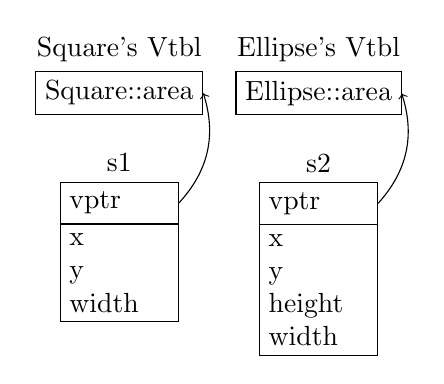
\begin{tikzpicture}[%
  object/.style={rectangle split,
                 fill=white,
                 draw
  }
]
\node [object, rectangle] (Avtbl) {
   Square::area
   };
\node [above] at (Avtbl.north) {Square's Vtbl};

\node [object, anchor=north, rectangle] (Bvtbl)
   at ($(Avtbl.north) + (right:6pc)$) {
   Ellipse::area
   };
\node [above] at (Bvtbl.north) {Ellipse's Vtbl};

\node [object, rectangle split parts=2, anchor=north,text width=3pc] (s1)
   at ($(Avtbl.south) + (down:2pc)$) { vptr \\
    \nodepart{second} x \\
 y \\
 width
};
\node [above] at (s1.north) {s1};
\draw [->] (s1.text east) to [bend right] (Avtbl.east);

\node [object, rectangle split parts=2, anchor=north,text width=3pc] (s2)
   at ($(Bvtbl.south) + (down:2pc)$) { vptr
    \nodepart{second} x \\
 y \\
 height \\
 width
    };
\node [above] at (s2.north) {s2};
\draw [->] (s2.text east) to [bend right] (Bvtbl.east);


   
\end{tikzpicture}

When \emph{area} is called, the runtime follows the object's virtual
table pointer (first field in the object) and jumps to the first
function pointer in the list (``area'').

\fi

\vspace{5pc}

\item (20 pts.)  For the program below written in a C-like language
  with nested function definitions,

  \begin{minipage}{0.4\textwidth}
\begin{lstlisting}
void main() {
  int x = 5;
  
  void bar() {
    x = x + 2;
  }
  
  void foo() {
    int x = 8;
    bar();
    printf("%d\n", x);
  }
  
  foo(); /* Body of main() */
}
\end{lstlisting}
  \end{minipage}%
  \begin{minipage}{0.6\textwidth}
    What would it print if the language used \textbf{static scoping}?   
    \field[height=3pc,width=3pc,multiline=false]{5a}

    \vspace{2pc}

    What would it print if the language used \textbf{dynamic scoping}?    
    \field[height=3pc,width=3pc,multiline=false]{5b}
  \end{minipage}

\ifkey
Static scoping: 8 \quad \emph{bar} doesn't change local \emph{x}\\
Dynamic scoping: 10 \quad \emph{bar} changes 8 into 10 \\
\fi

\end{enumerate}

\end{Form}

\end{document}

% Local Variables:
% compile-command: "make hw3.pdf"
% End:
